\documentclass[10pt,a4paper]{article}

% ─── Packages ─────────────────────────────────────────

\usepackage{fontspec}
\setmainfont{Times New Roman}

\usepackage[top=1.1cm,bottom=1.1cm,left=1.55cm,right=1.55cm]{geometry}

\usepackage{titlesec}
\usepackage{enumitem}
\usepackage{hyperref}
\usepackage{xcolor}
\usepackage{tabularx}
\usepackage{graphicx}
\usepackage{parskip}

% ─── Colors ───────────────────────────────────────────

\definecolor{primary}{RGB}{30,40,90}
\definecolor{namecolor}{RGB}{0,120,180}
\definecolor{accent}{RGB}{50,90,150}
\definecolor{rulecol}{RGB}{200,205,220}
\definecolor{gray}{RGB}{90,90,90}

\hypersetup{
    colorlinks=true,
    urlcolor=accent
}

\pagestyle{empty}
\setlength{\parskip}{0pt}

% ─── Section ──────────────────────────────────────────

\titleformat{\section}
    {\normalsize\bfseries\color{primary}}
    {}
    {0em}
    {}
    [\vspace{1pt}\textcolor{rulecol}{\titlerule[0.6pt]}\vspace{1pt}]

\titlespacing{\section}{0pt}{5pt}{2pt}

% ─── Entry ────────────────────────────────────────────

\newcommand{\entry}[3]{%
    \noindent
    \begin{tabularx}{\linewidth}{X r}
        \textbf{\color{primary}#1} &
        {\scriptsize\color{gray}#2}
    \end{tabularx}\\[-2pt]
    {\scriptsize\textit{\color{gray}#3}}
    \vspace{1pt}
}

% ─── Compact list ─────────────────────────────────────

\newenvironment{cvitems}{
    \begin{itemize}[
        leftmargin=1.15em,
        topsep=0pt,
        itemsep=0.5pt,
        parsep=0pt,
        partopsep=0pt
    ]
}{
    \end{itemize}
}

% ═════════════════════════════════════════════════════

\begin{document}

% ─── HEADER ───────────────────────────────────────────

\noindent
\begin{tabularx}{\linewidth}{@{}X r@{}}

\begin{minipage}[c]{\linewidth}

    {\LARGE\bfseries\color{namecolor} Ho Huynh Nhu}\\[2pt]

    {\large\bfseries\color{primary}
    AI Engineer}\\[3pt]

    {\scriptsize\color{gray}
    20/10/2003
    \enspace\textcolor{rulecol}{|}
    \enspace (+84) 367 503 477
    \enspace\textcolor{rulecol}{|}
    \enspace
    \href{mailto:hhnhu2003@gmail.com}{hhnhu2003@gmail.com}
    \enspace\textcolor{rulecol}{|}
    \enspace Ho Chi Minh City}\\[2pt]

    {\scriptsize
    \href{https://github.com/hohuynhnhu}
    {github.com/hohuynhnhu}
    \enspace\textcolor{rulecol}{|}
    \enspace
    \href{https://www.facebook.com/huynhnhu.ho.961}
    {facebook.com/huynhnhu.ho.961}
    }

\end{minipage}

&

\begin{minipage}[c]{2.2cm}
    \raggedleft
    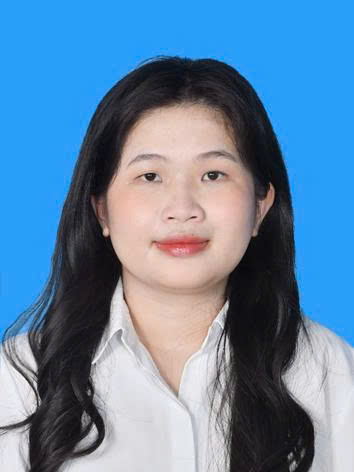
\includegraphics[
        width=2.2cm,
        height=2.7cm,
        keepaspectratio
    ]{assets/avt.jpg}
\end{minipage}

\end{tabularx}

\vspace{3pt}
\textcolor{rulecol}{\rule{\linewidth}{0.6pt}}

% ─── CAREER OBJECTIVE ─────────────────────────────────

\section*{Career Objective}

{\small
Final-year Information Technology student pursuing an AI Engineer
career, with hands-on experience in Computer Vision, Deep Learning,
and Python-based AI systems. Experienced in developing, training,
evaluating, and integrating AI models including YOLO, CNN, Siamese
Networks, MediaPipe, and Transformer. Seeking an AI Engineer position
to apply machine learning knowledge to real-world products and
continue developing expertise in AI model development and deployment.
}

% ─── EDUCATION ────────────────────────────────────────

\section*{Education}

\entry
{University of Transport Ho Chi Minh City (UTH)}
{10/2022 -- 10/2026}
{Bachelor of Information Technology -- Completed coursework}

{\small
\begin{cvitems}
    \item GPA: 3.4 / 4.0
    \item \textbf{Excellent Scholarship} -- Semester 1, 2025
    \item \textbf{Second Prize -- AI Track},
    UTH Student Scientific Research Conference 2025
\end{cvitems}
}

% ─── AI / TECHNICAL SKILLS ────────────────────────────

\section*{Technical Skills}

{\small
\begin{tabularx}{\linewidth}{@{}lX@{}}

\textbf{AI / Machine Learning}
&
Machine Learning, Deep Learning, Computer Vision,
CNN, YOLO, Siamese Network, Transformer
\\[1.5pt]

\textbf{Computer Vision}
&
Object Detection, Pose Estimation, Image Classification,
Face Recognition, Image Processing, MediaPipe
\\[1.5pt]

\textbf{AI Development}
&
Python, PyTorch, OpenCV, Ultralytics YOLO,
FastAPI, NumPy, Pandas
\\[1.5pt]

\textbf{AI Models}
&
YOLOv8, YOLO Pose, CNN, Siamese Network,
Transformer Encoder, ArcFace, MediaPipe
\\[1.5pt]

\textbf{Backend / API}
&
Python, FastAPI, Node.js, RESTful API
\\[1.5pt]

\textbf{Database / Data}
&
PostgreSQL, SQL Server, MongoDB, Firebase,
Supabase, dbt, Airflow
\\[1.5pt]

\textbf{Tools}
&
Git, Docker, Postman, VS Code, Power BI
\\[1.5pt]

\textbf{Programming}
&
Python, SQL, TypeScript, JavaScript, Kotlin
\\[1.5pt]

\textbf{English}
&
Technical document reading and basic professional communication

\end{tabularx}
}

% ─── WORK EXPERIENCE ──────────────────────────────────

\section*{Work Experience}

\entry
{Gotik Consulting -- Data Engineer}
{Python \textbar{} dbt \textbar{} PostgreSQL \textbar{} Airflow}
{03/2026 -- 05/2026}

{\small
\begin{cvitems}
    \item Processed and transformed Odoo data for analytics and
    reporting workflows.
    
    \item Developed Python-based data pipelines and data models
    using dbt and Neon PostgreSQL.
    
    \item Automated hourly data processing workflows with
    Apache Airflow.
    
    \item Prepared structured datasets for analysis and developed
    Power BI dashboards for operational monitoring.
\end{cvitems}
}

% ─── PROJECTS ─────────────────────────────────────────
\section*{Featured AI Projects}

\entry
{Fall Detection -- Real-Time AI Fall Detection System}
{Python \textbar{} YOLOv8 Pose \textbar{} MediaPipe \textbar{} Transformer \textbar{} FastAPI}
{04/2026 -- 06/2026}

{\small
\begin{cvitems}
    \item Developed a real-time fall detection system using YOLOv8 Pose, MediaPipe, and Transformer.
    \item Trained a Transformer Encoder with 30-frame $\times$ 200-feature input for fall/non-fall classification.
    \item Achieved 97.8\% mean accuracy with 5-fold cross-validation and integrated FastAPI for real-time alerts.
    \item GitHub: \href{https://github.com/hohuynhnhu/Fall-Detection}{Fall-Detection}
\end{cvitems}
}

\vspace{3pt}

\entry
{VehicleScan -- Smart Parking System with AI \& IoT}
{Python \textbar{} YOLO \textbar{} CNN \textbar{} Siamese Network \textbar{} ESP32}
{03/2025 -- 03/2026}

{\small
\begin{cvitems}
    \item Developed vehicle detection and recognition models using YOLO, CNN, and Siamese Network.
    \item Prepared datasets and trained AI models for real-time vehicle identification.
    \item Integrated AI models with ESP32 and Firebase; won Second Prize -- AI Track at UTH 2025.
    \item GitHub: \href{https://github.com/LeKhang-cn22h/VehicleScanner.git}{VehicleScanner}
\end{cvitems}
}

% ─── ADDITIONAL INFORMATION ───────────────────────────

\section*{Additional Information}

{\small
\begin{tabularx}{\linewidth}{@{}lX@{}}

\textbf{Soft Skills}
&
Problem-solving \textbar{}
Research and self-learning \textbar{}
Teamwork \textbar{}
Troubleshooting
\\[2pt]

\textbf{AI Interests}
&
Computer Vision \textbar{}
Deep Learning \textbar{}
AI Model Development \textbar{}
Real-time AI Systems
\\[2pt]

\textbf{Other}
&
Experience integrating AI models with APIs,
databases, IoT devices, and real-time applications.
\\[2pt]

\textbf{Availability}
&
Available for full-time AI Engineer opportunities
and willing to adapt to job requirements.

\end{tabularx}
}

\end{document}